% Chapter 6

\chapter{Evaluation}% Main chapter title

\label{Chapter6} % For referencing the chapter elsewhere, use \ref{Chapter6} 
In this chapter, experiments are performed to determine whether the propositions of the database model and the database application design in Chapter 4 and Chapter 5 meet the user requirements. The experiments are real-time data collection and an overnight data collection, importing data from EDF file format, exporting data from the database to EDF file format, and querying data from the database. When performing a database evaluation, the most important metrics to evaluate are the read/write speed and the size of the database, because the time to retrieve data and space to store data must meet the user requirements. Moreover, the database application must ensure that no data is lost or data corrupted when storing and retrieving data. With respect to mobile platforms, which are usually limited resources and battery driven, the database application must also use the resources in an efficient way.\\
The extensibility for future usage is clearly presented in the design chapter, and therefore not be evaluated in this section. As discussed in the design chapter, the database design is platform independent, it can easily be implemented on a bio-signals collector application such as CESAR acquisition tool to minimize the sending and receiving overhead between collectors and the database application server. There are some common experiments when evaluating a database design and database application. However, the experiments in this chapter are chosen to prove that the database model and database application are good candidates to be used to store OSA data on a mobile device. Therefore, experiments on storing real time data, overnight experiment, import and export to EDF files are performed in this section. In addition, a stress test experiment is performed to find the limited of the database application with respect to the resource usage and the number of channels it can manage.\\
The goals of the experiments are to evaluate the feasibility of the database model, and to convince the reader that the functional and non-functional requirements for the database modeling and the database application are satisfied by measuring performance of the read/write on the database, performance of the database application, and storage capacity. In this section, each experiment is described with respect to the reasons why it is performed, which workloads are used, which metrics are studied, the experiment itself, and the results from the experiment.\\
A BITalino plugged kit, two Android devices, and a CESAR acquisition simulator run on macOS Sierra are used for the experiments. Table \ref{tab:DevicesSpecs} presents the specifications of these devices.
\section{Real-time data collection experiment}
\begin{table}
\begin{center}
\begin{tabular}{ |p{2cm}|p{2.7cm}|p{2.8cm}|p{3cm}|}
 \hline
 \cellcolor[HTML]{00D2CB}Technology&\cellcolor[HTML]{00D2CB}Xiaomi Mi5& \cellcolor[HTML]{00D2CB}MacBook Retina\newline 15 Late 2013&\cellcolor[HTML]{00D2CB}BITalino BT\newline plugged kit\\
 \hline
 \cellcolor[HTML]{00D2CB}OS&Android 7.0& macOS Sierra&n/a\\
 \hline
 \cellcolor[HTML]{00D2CB}RAM&3GB&16GB&n/a\\
 \hline
 \cellcolor[HTML]{00D2CB}CHIP&Snapdragon 820\newline 4 core 1.8GHz&Intel core i7\newline 4 core 2.3GHz&MCU with sampling rate 1, 10, 100, or 1000Hz\\
 \hline
 \cellcolor[HTML]{00D2CB}Wi-Fi&802.11\newline a/b/g/n/ac& 802.11\newline a/b/g/ac&n/a\\
 \hline
 \cellcolor[HTML]{00D2CB}Bluetooth&v4.2&v4.0&v2.0, range 10m\\
 \hline
 \cellcolor[HTML]{00D2CB}Battery&3000mAh&8440mAh&500mAh or 1500mAh\\
 \hline
\end{tabular}
\end{center}
\caption{Used devices specifications}
\label{tab:DevicesSpecs}
\end{table}
The database application is required to collect and store bio-signal data from the CESAR acquisition tool to the designed database model on a mobile device. The CESAR acquisition tool can send data with four different frequencies to the database, that are 1Hz, 10Hz, 100Hz, and 1000Hz. The goal of the database application is to collect OSA data. The application should be used for sleep monitoring to collect OSA data, which can last more than 8-10 hours. Therefore, We perform some experiments with a duration of more than 12 hours. To prove that the application properly works for a long time collection, an overnight experiment is presented in the next section. Currently, the CESAR acquisition tool cannot delivery samples at 1000Hz, it stops sending data after 30min-40min. Therefore, a CESAR acquisition simulator is used for sending samples with frequencies 1000Hz or higher. Goals of this experiment are to evaluate the database read/write performances and database size when collecting data from many different sources with different frequencies. Since the application is run on a mobile platform where the resources are limited, usage resources such as CPU and battery consumption are also evaluated in this section.
\subsection{Experiment workloads}
The database application collects samples from multiple sources simultaneously, in which each source sends data at different frequencies. The amount of samples the database needs to store at a certain time is depending on the number of currently connected sources and the number of channels that belong to each source. In addition, when the frequencies are high, the number of arriving samples in a time period becomes very large; which in turn has a huge impact on the storing process of the database application. Since the application uses batch processing to manage and store incoming samples, the batch size strongly influences the performance of the application. The batch size is defined by multiplying the buffer duration with the arrival rate. Therefore, the workloads for the experiment are the buffer duration in second, the arrival rate of a source in Hz, and the number of channels (total channels from the connected sources).
\subsection{Experiment metrics}
Evaluation metrics must be meaningful to analyze whether the user requirements can be fulfilled. In the real-time data collection experiment, the application has to parse incoming data packets and transform them into useful objects for the database. The percent CPU usage and power consumption are considered the metrics used in the evaluation, because the application needs to create object for each incoming sample, then checking if the current batch must be sent to the thread that manages the database insertion. Percentage of CPU usage is obtained by using command “adb shell busybox top –d 5”. This command generates an output which contains the information about CPU usage for each application, and the output is printed in the standard output in every five seconds. The outputs from the command are redirected to a text file, and the file is presented in charts. The python code for parsing CPU usage texts file into a chart is presented in Appendix \ref{AppendixC}, in which Listing \ref{listing:BUSYBOXTOPTEXT} presents a sample output from the command, and a discussion about how to parse the output is also illustrated in the appendix. Power consumption can be obtained after a collection process is finished by using a built-in battery management application of the Android system (Settings - Battery - Battery use). Figure \ref{fig:Figures/PowerMetric} presents an overnight experiment sample where the power consumption for each application is calculated in percent of the total power drained off.\\
Since the application uses batch processing to manage the incoming data, the SQLite transaction is requested for inserting data into the database when the temporary buffer is full. While the transaction is performed, it locks the entire database file. Hence, the SQLite time usage in millisecond for different batch sizes, and the number of insertions per millisecond are another metrics for the experiment. Since the application is implemented on the mobile platform where resources are limited, it is good to see how big the database grows in megabytes for different workloads in a specific period time.
\subsection{Experiment setup}
As described above, there are two workload generators that are used in the experiment, they are the CESAR acquisition tool, and the CESAR acquisition simulator. In addition, a control parameter which is the buffer duration for the application can be adjusted before performing a collecting process. A control parameter is a value that is adjusted before a collecting process starts is named the experimental workload. Calculated results after each collection process are named the responsive metrics in the tables that are used in this section.\\
Table \ref{tab:BufferDuration} presents the responsive metrics for an experiment where the experimental workload is a buffer duration; control workloads are arrival rate and number of used channels. In this experiment, arrival rate is 100Hz, and all channels of the CESAR acquisition tool are used (6 channels). Likewise, in Table \ref{tab:ArrivalRate}, the experimental workload is arrival rate; control workloads are buffer duration (10 second), and all channels of the CESAR acquisition tool are used (6 channels). The number of channels is chosen as the experimental workload in Table \ref{tab:NrOfChannels}. In this case, the control workloads are the buffer duration (10s) and arrival rate (100Hz).\\
For each experiment, a data collection process is iterated three times with a specific experimental workload value. That is, experimental workloads for the buffer duration (batch size) are 10 seconds, 20 seconds, and 30 seconds; experimental workloads for the arrival rate are 1Hz, 10Hz, 100Hz, and 1000Hz; experimental workloads for number of channels are 1 channels, 3 channels and 6 channels. The metrics that are evaluated for these iterations are the power consumption, SQLite usage time, and the size of the database after the iterations.\\
The duration for each iteration is about 60 minutes. Because the main metrics for the experiment are the SQLite write performance, resource usage, and the size of the collected data in the database, it does not need to perform a long time run for each iteration. Instead, only one overnight experiment is performed to demonstrate that the database application is to store all data from a long time run. The Xiaomi Mi5 phone is connected to the MacBook via a USB cable such that the percentage of CPU usage of the phone are sent to the MacBook. That is, an adb shell busybox command is run on the Terminal of the MacBook, and the percentage of CPU usage from the adb are redirected to a text file which is stored in the root of the folder project of the database application. The percentage of power consumption is obtained from the "Battery use" of the Android operating system. However, the iteration needs to be repeated without connecting to the MacBook or a power adapter since the "Battery use" does not perform the calculation unless the phone is powered by the battery. The database size in megabytes is obtained by getting the length of the database file, then dividing for 1024*1024 (converting from byte to megabyte). Listing \ref{listing:GETDBSIZE} presents how to get the SQLite database size in the Android device. To calculate SQLite time usage, a timer is set before each SQL insert transaction. That is, the timer is started and stopped for each SQLite query execution, then the total SQLite time usage is obtained by adding all results from the executions.
\begin{table}
\centering
\begin{tabular}{|l|r|r|r|}
\hline
\multicolumn{1}{|c|}{\cellcolor[HTML]{00D2CB}} & \multicolumn{3}{c|}{\cellcolor[HTML]{00D2CB}\begin{tabular}[c]{@{}c@{}}Experimental workload in 60 min \\ Buffer duration\end{tabular}} \\ \cline{2-4} 
\multicolumn{1}{|c|}{\multirow{-2}{*}{\cellcolor[HTML]{00D2CB}Responsive metrics}} & \multicolumn{1}{l|}{\cellcolor[HTML]{00D2CB}10 seconds} & \multicolumn{1}{l|}{\cellcolor[HTML]{00D2CB}20 seconds} & \multicolumn{1}{l|}{\cellcolor[HTML]{00D2CB}30 seconds} \\ \hline
\cellcolor[HTML]{00D2CB}\begin{tabular}[c]{@{}l@{}}CPU usage \\ (percent with 5s segment)\end{tabular} & \multicolumn{1}{c|}{RTbd1.txt} & \multicolumn{1}{c|}{RTbd2.txt} & \multicolumn{1}{c|}{RTbd3.txt} \\ \hline
\cellcolor[HTML]{00D2CB}\begin{tabular}[c]{@{}l@{}}Power consumption\\ (percent)\end{tabular} & 2.5 & 2.6 & 2.4 \\ \hline
\cellcolor[HTML]{00D2CB}\begin{tabular}[c]{@{}l@{}}SQLite time usage\\ (millisecond)\end{tabular} & 194 242 & 193 130 & 184 811 \\ \hline
\cellcolor[HTML]{00D2CB}\begin{tabular}[c]{@{}l@{}}Duration\\ (millisecond)\end{tabular} & 3 668 780 & 3 750 028 & 3 711 576 \\ \hline
\cellcolor[HTML]{00D2CB}\begin{tabular}[c]{@{}l@{}}Database size\\ (Megabytes)\end{tabular} & 90 & 91 & 91 \\ \hline
\end{tabular}
\caption{Buffer duration}
\label{tab:BufferDuration}
\end{table}
\begin{table}
\centering
\begin{tabular}{|l|c|c|c|l|}
\hline
\multicolumn{1}{|c|}{\cellcolor[HTML]{00D2CB}} & \multicolumn{4}{c|}{\cellcolor[HTML]{00D2CB}\begin{tabular}[c]{@{}c@{}}Experimental workload in 60 min \\ Arrival rate\end{tabular}} \\ \cline{2-5} 
\multicolumn{1}{|c|}{\multirow{-2}{*}{\cellcolor[HTML]{00D2CB}Responsive metrics}} & \multicolumn{1}{l|}{\cellcolor[HTML]{00D2CB}1 Hz} & \multicolumn{1}{l|}{\cellcolor[HTML]{00D2CB}10 Hz} & \multicolumn{1}{l|}{\cellcolor[HTML]{00D2CB}100 Hz} & \cellcolor[HTML]{00D2CB}700 Hz (simulator) \\ \hline
\cellcolor[HTML]{00D2CB}\begin{tabular}[c]{@{}l@{}}CPU usage\\ (percent with 5s segment)\end{tabular} & RTar1.txt & RTar2.txt & RTar3.txt & RTar4.txt \\ \hline
\cellcolor[HTML]{00D2CB}\begin{tabular}[c]{@{}l@{}}Power consumption\\ (percent)\end{tabular} & <1 & <1 & 2.5 & 2.7 \\ \hline
\cellcolor[HTML]{00D2CB}\begin{tabular}[c]{@{}l@{}}SQLite time usage\\ (millisecond)\end{tabular} & 14 311 & 39 442 & 194 242 & 2 012 042 \\ \hline
\cellcolor[HTML]{00D2CB}\begin{tabular}[c]{@{}l@{}}Duration\\ (millisecond)\end{tabular} & 3 658 002 & 3 679 001 & 3 668 780 & 3 737 474 \\ \hline
\cellcolor[HTML]{00D2CB}\begin{tabular}[c]{@{}l@{}}Database size\\ (Megabytes)\end{tabular} & < 1 & 9 & 90 & 653 \\ \hline
\end{tabular}
\caption{Arrival rate}
\label{tab:ArrivalRate}
\end{table}
\begin{table}
\centering
\begin{tabular}{|l|c|c|c|}
\hline
\multicolumn{1}{|c|}{\cellcolor[HTML]{00D2CB}} & \multicolumn{3}{c|}{\cellcolor[HTML]{00D2CB}\begin{tabular}[c]{@{}c@{}}Experimental workload in 60 min \\ Number of channels\end{tabular}} \\ \cline{2-4} 
\multicolumn{1}{|c|}{\multirow{-2}{*}{\cellcolor[HTML]{00D2CB}Responsive metrics}} & \multicolumn{1}{c|}{\cellcolor[HTML]{00D2CB}1} & \multicolumn{1}{c|}{\cellcolor[HTML]{00D2CB}3} & \multicolumn{1}{c|}{\cellcolor[HTML]{00D2CB}6} \\ \hline
\cellcolor[HTML]{00D2CB}\begin{tabular}[c]{@{}l@{}}CPU usage\\ (percent with 5s segment)\end{tabular} & RTnrc1.txt & RTnrc3.txt & RTnrc6.txt \\ \hline
\cellcolor[HTML]{00D2CB}\begin{tabular}[c]{@{}l@{}}Power consumption\\ (percent)\end{tabular} & 1.5 & 2.2 & 2.5 \\ \hline
\cellcolor[HTML]{00D2CB}\begin{tabular}[c]{@{}l@{}}SQLite time usage\\ (millisecond)\end{tabular} & 54 613 & 113 050 & 194 242 \\ \hline
\cellcolor[HTML]{00D2CB}\begin{tabular}[c]{@{}l@{}}Duration\\ (millisecond)\end{tabular} & 3 678 704 & 3 675 105 & 3 668 780 \\ \hline
\cellcolor[HTML]{00D2CB}\begin{tabular}[c]{@{}l@{}}Database size\\ (Megabytes)\end{tabular} & 15 & 44 & 90 \\ \hline
\end{tabular}
\caption{Number of channels}
\label{tab:NrOfChannels}
\end{table}
\begin{minipage}{\linewidth}{}
\begin{lstlisting}[caption={Get the size of a SQLite database in the Android}, label = {listing:GETDBSIZE}, captionpos=b, basicstyle=\ttfamily\footnotesize]
File f = getApplicationContext().getDatabasePath(OSADBHelper.DATABASE_NAME);
long dbSize = f.length()/(1024*1024);
Toast.makeText(getApplicationContext(),"Database size "+String.valueOf(dbSize)
               +" MB",Toast.LENGTH_SHORT).show();
\end{lstlisting}
\end{minipage}
\subsection{Results and discussion}
As presented in Table \ref{tab:BufferDuration}, \ref{tab:ArrivalRate}, and \ref{tab:NrOfChannels}, the power consumption is about 2.5\% with arrival rates smaller than 100Hz. That is, the database application does not consume much battery, because the CPU time used to parse the arrival samples is low. The experiments, where the buffer duration and the number of channels are used as experimental workloads, illustrates that the power consumption and the CPU usage have a small variation. It is because the arrival rate for these experiments is the same. The variation occurs in these experiments since different buffer durations and number of channels causes different overhead when inserting samples to the database. Therefore, the power consumption and CPU usage are mainly depending on the arrival rate, the higher the arrival rates, the more time the CPU time it takes to parse the arrival samples, hence the more power is drained.\\
The write performance of the database application does not depend on the arrival rate and the number of channels, it is mainly depending on the size of the buffer (the batch) that groups all arrival samples into a insert transaction. In theory, the more samples in groups, the less time is needed for writing to the database. However, the performance of the database application is not increased so much. As presented in Table \ref{tab:BufferDuration}, tripled the buffer duration, the performance is increased (184811*100\%)/194242 which is about 9.5\%. Therefore, a fixed duration of the buffer is recommended to use for the database application on the Android platform.\\
As presented in Table \ref{tab:ArrivalRate}, and \ref{tab:NrOfChannels}, the size of the database is depending on the arrival rate and the number of channels that are used to collect samples. If sensor kits deliver data tuples with a frequency of 1Hz, the database can continuously store data for six channels up to 41 days by using 1GB memory, that is, one megabyte per hour which is 1000 hours for 1GB or about 41 days. Hence, the Xiaomi phone that is used in the thesis can continuously collect and keep data for 20GB * 41 days = 820 days, or 2,2 years without backing up to a stationary computer. However, high frequencies offer better data for later analysis, hence, 10Hz, 100Hz and 250Hz are often used to collect bio-physiological signals. The size of the database is linearly increasing when the frequency is increased. With frequencies from 100Hz to 700Hz, the collected data needs to be backed up to a stationary computer after one or two overnight collections.\\
\section{Overnight experiment}
An overnight experiment is performed in this thesis to demonstrate that the database application can collect data for a long period period of time. In addition, the feasibility of the database model and database application for monitoring sleep during a whole night is also analyzed by assessing metrics such as the power usage, the size of the collected data, time that the database application accesses the database file, etc. In this experiment, the database application receives data from the CESAR acquisition tool until the tool or a users disconnects the connection.
\subsection{Experiment workloads and metrics}
Workloads that are used in this experiment, are all channels from the BITalino sensor kit (6 channels). Each channel collects data with 100Hz frequency, which is 100 samples per second. Therefore, the number of samples the database application needs to put to the database in one second is 600 samples. To avoid overhead when accessing the database file for storing samples, the database application uses batch processing. The batch size that is used in this experiment is 5 seconds. That is, the application groups 5*600 = 3000 samples into one insert transaction (instead of 3000 transactions if the batch processing is not used). The metrics used in for this experiment are the percentage of power consumption of the total power usage of the mobile device, size of the collected data in megabytes, number of samples in the database, number of received packets, percent time accessing the database file over the experiment duration.
\subsection{Experiment setup}
The BITalino can be powered by different battery capacities; a 500mAh and 1500mAh, which can offer about 6 to 20 hours for collecting data with 100Hz each channel. However, only the 1500mAh battery is used in this experiment, because early tests showed that the 500mAh battery can not be used for performing the overnight experiment. The 1500mAh battery of the BITalino sensor kit is full charged before the experiment. In addition, the Xiaomi Mi5 phone is plugged to a power adapter, because the current version of the CESAR acquisition tool needs the display of the phone to be on to avoid to be killed by the Android system because it is running for a long time. This configuration does not impact the experiment, since the metric that is used for evaluating the power usage, is the percentage of power the application consumed over the total used power during the experiment. The phone is full charged and disconnected from the power adapter before the experiment, then the percentage of power consumption of the database application is gotten from the built-in battery management application of the Android operating system when the battery power is about 50\%. In other words, the percentage of power usages for applications, which are running under the experiment, are stable, therefore, the power usage of the database application can be evaluated without waiting for the battery of the phone is run out. After obtaining the percentage of the power usage, the phone is connected to the power adapter to continue the collection process. The total SQLite time usage is calculated by adding all timed insertions of each transaction from the batch processing. The duration is calculated by subtracting the maximum timestamp and the minimum timestamp of the samples in the overnight record. The percentage of power consumption is gotten from the built-in battery management application, which is named "Battery use", of the Android operating system. The number of packets can be gotten from either the CESAR acquisition tool, or counting number of samples in the database dividing to number of channels that are used in the experiment (6 channels). To get the number of collected samples, a simple SQL query is performed, i.e., "SELECT COUNT(*) FROM SAMPLE". Since the database is empty before the experiment is performed, the database size is also the size of all data collected after the experiment performed. The results from the experiment are presented in Table \ref{tab:OvernightExperiment}.
\begin{table}
\centering
\begin{tabular}{|l|r|}
\hline
\cellcolor[HTML]{00D2CB}Start time & 20.04.2017 17:43:55 \\ \hline
\cellcolor[HTML]{00D2CB}End time & 21.01.2017 12:32:20 \\ \hline
\cellcolor[HTML]{00D2CB}Duration & 67 705 166ms = about 18 hours, 48min \\ \hline
\cellcolor[HTML]{00D2CB}\begin{tabular}[c]{@{}l@{}}SQLite time usage\\ (millisecond)\end{tabular} & 4 251 412 ms \\ \hline
\cellcolor[HTML]{00D2CB}\begin{tabular}[c]{@{}l@{}}Percent SQLite time usage\\ over the duration\end{tabular} & 4 251 412/ 67 705 166 = about 6.3\% \\ \hline
\cellcolor[HTML]{00D2CB}\begin{tabular}[c]{@{}l@{}}Power consumption\\ (percent)\end{tabular} & 6.6\% of total power usage \\ \hline
\cellcolor[HTML]{00D2CB}\begin{tabular}[c]{@{}l@{}}Number packet\\ from the CESAR\\ acquisition tool\end{tabular} & 6 770 896 packets \\ \hline
\cellcolor[HTML]{00D2CB}Number of samples & 40 625 376 \\ \hline
\cellcolor[HTML]{00D2CB}\begin{tabular}[c]{@{}l@{}}Database size\\ (Megabytes)\end{tabular} & 1736 MB \\ \hline
\end{tabular}
\caption{Overnight experiment}
\label{tab:OvernightExperiment}
\end{table}
\subsection{Results and discussion}
For the write performance of the database application, as presented in Table \ref{tab:OvernightExperiment}, the number of samples are that collected during the experiment is 40625376, and the total time used for the insert transactions is 4251412 millisecond. Based on these numbers, the average time used for each transaction is 4251412/(40625376/3000) = 314 millisecond, where 40625376/3000 = 13542 is the total number of insert transactions performed. That is, the database uses 314 millisecond to store samples from 5000 millisecond (5 second buffer). Hence, the percent time usage for accessing the database file (I/O time usage) is (314/5000)*100\% which is about 6.3\% of the idle, it can also be calculated by using the total SQLite time usage and the duration as presented in Table \ref{tab:OvernightExperiment}. Based on the percent time usage, the database application can manage up to 15 BITalino sensor kits where all channels of the kits are used, and the I/O time usage to access the database file would be 15*6.3\% = 94,5\% idle. 15 BITalino sensor kits offer 15*6 = 90 different sensors that can be used to collect data at 100Hz, or 15 users can use one Xiaomi MI5 phone to store data simultaneously.\\
\begin{figure}
    \centering
    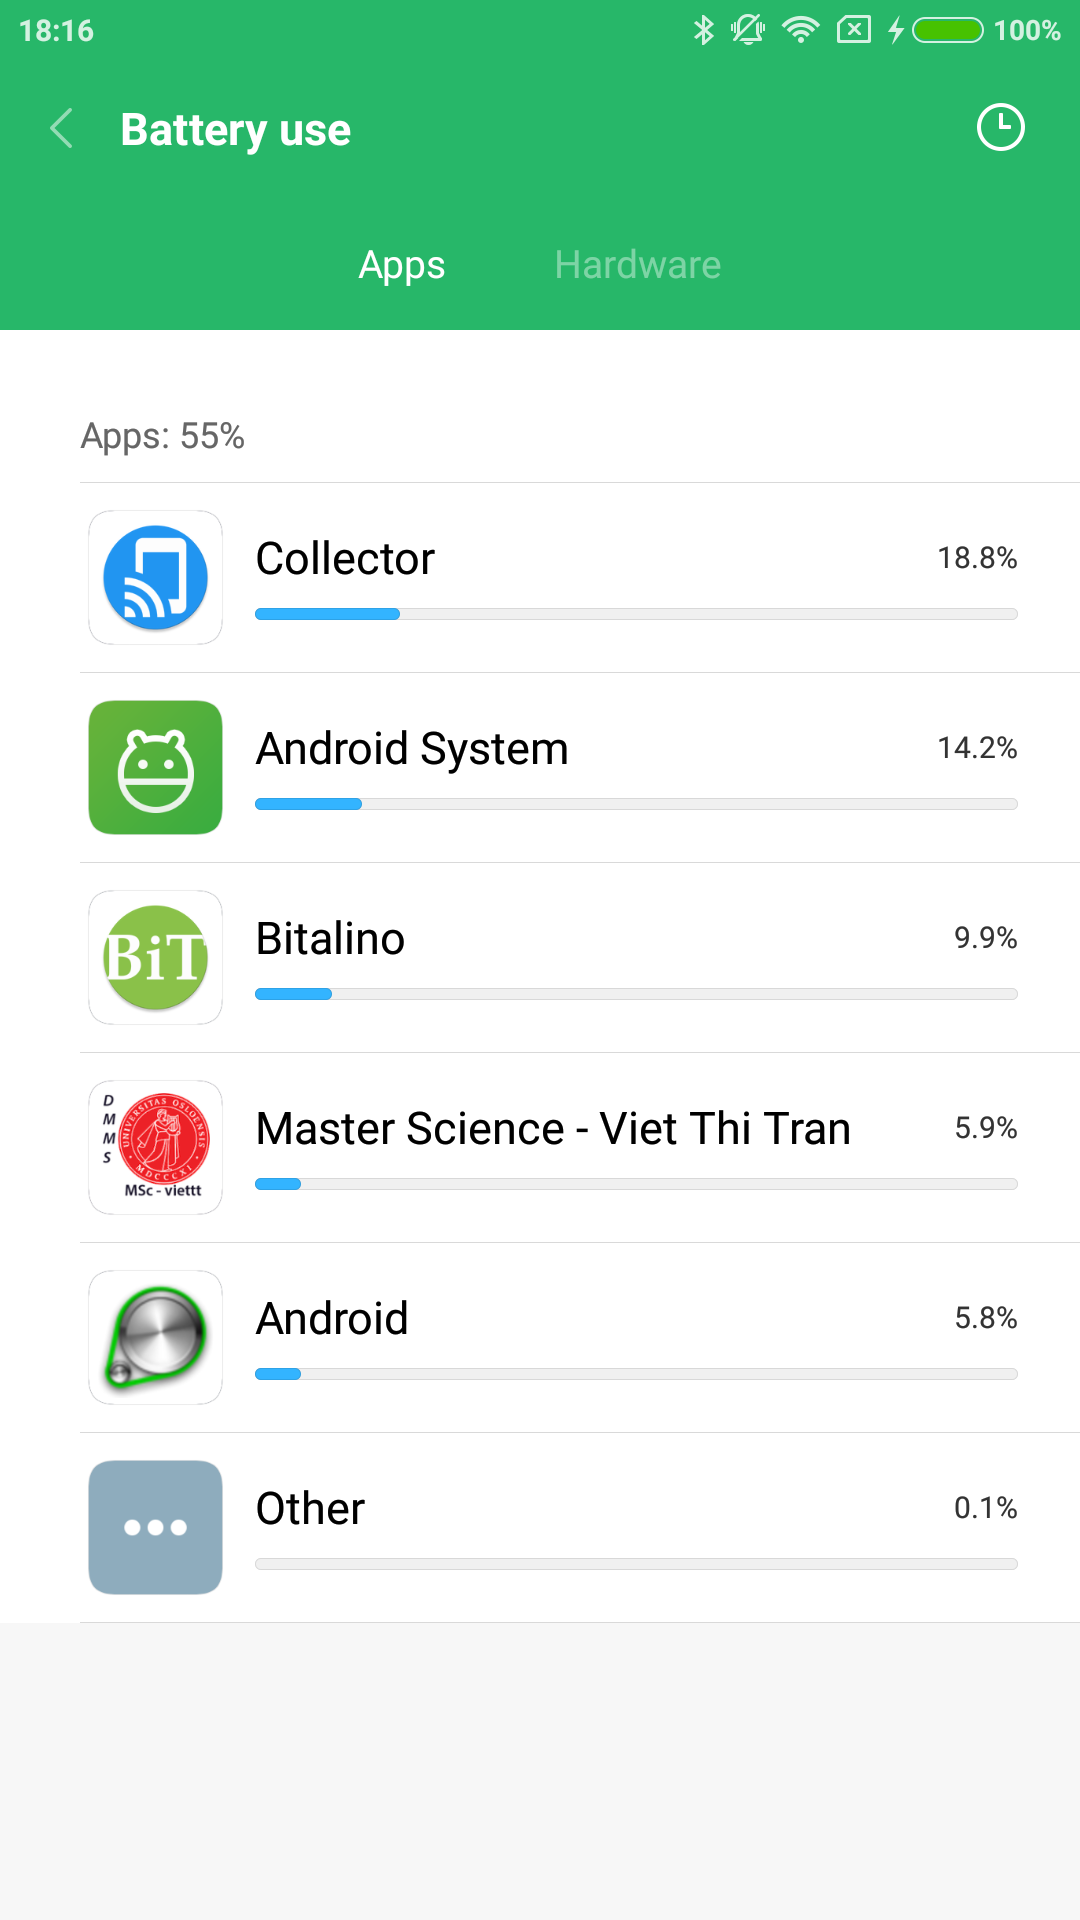
\includegraphics[width=0.4\textwidth]{Figures/PowerMetric.png}
    \caption{Battery usage under overnight experiment}
    \label{fig:Figures/PowerMetric}
\end{figure}
For the power consumption, the database application does not use much battery compared to other applications. Figure \ref{fig:Figures/PowerMetric} presents the power consumption for applications that are running during the experiment. The CESAR acquisition tool consumes about 31.1\% while the database application consumes 6.6\% of total power usage. Hence, the application is considered quite efficient in the case of power usage.\\
The overnight experiment is performed during 18 hours and 48 minutes, which is longer than a normal nighttime sleep. The data size after collecting data for nearly 19 hours is 1736 megabytes (1.7 GB). Currently, an Android phone usually has 16 to 64 gigabytes(GB) internal memory, in addition, an external Secure Digital (SD) card with 16GB costs about 80kr. With a 16GB SD card, a user can store up to nine 18 hours (overnight) records, or nine users can use the same SD card to store their collected data. The phone that is used in the experiment has 32GB memory which offers 15 users use it simultaneously. It is 15 users, because the write performance from the previous discussion can handle up to 15 users.\\
Nonetheless, the results from the experiment present that the database application is properly good to be used for a long period time of data collection. Moreover, multiple users can share an Android mobile device to store their data. Furthermore, the power consumption and data size are properly good enough when collecting data for a long period of time.
\section{EDF import}
The database model is designed in a way that opens for all bio-signals, and can store data from other database sources if the sources support EDF exporting. In other words, the data base application is required to import data from EDF and EDF+ file formats. Goals of the experiment are to evaluate database writing performance and usage resources such as CPU and battery consumption, especially, when the application reads files simultaneously.
\subsection{Experiment workloads}
The database application reads data samples from multiple files simultaneously. Ideally, each sample from the files is parsed to an object in memory, then inserted into the database. However, each INSERT statement in SQLite has its own transaction, and SQLite can only do a few dozen transactions per second. The samples are, therefore, grouped into a transaction before performing a SQLite insertion. The transaction locks the entire database file when it inserts the data. Hence, if the sample group is too large, it can cause either a memory problem, or poor performance since other transactions have to wait for it. Therefore, the workloads for the experiment are the size of the sample group and the number of file reads.
\subsection{Experiment metrics}
Metrics that are chosen to highlight the goals and workload of the experiment are the percentage of CPU usage, the percentage of power consumption, the size of a EDF file in the database, and the total time the experiment holds the shared SQLite connection. The percentage of CPU usage and the power consumption need to be evaluated since the application needs to parse the samples in the EDF file format to objects that can be stored into the database. In addition, the time that is used to insert samples can be used for evaluating the writing performance of the database.
\subsection{Experiment setup}
\begin{lstlisting}[caption={Convert mit2edf by using terminal}, label = {listing:MIT2EDF}, captionpos=b]
(no options)Terminal $mit2edf -r a01 
(options)Terminal $mit2edf -r a01 [-v -h -p] -o phy1.edf
\end{lstlisting}
To generate workloads for the experiment, a function from Physionet which is named mit2edf is used for exporting bio-signal data from Physionet databases to the EDF file format. As presented in the manual page of the function, mit2edf creates an EDF file that contains the same data as the input files which are in form of Waveform Database format (header and signal files). However, the function is included in the WFDB software package from Physionet, and the user must install the package first. There are three options when using the function which are printing a brief usage summary, choosing a name for the exported edf (the exported file has the same name as the imported record as default), and printing debugging output. Listing \ref{listing:MIT2EDF} presents how to use the function to convert a01 record to EDF file format without options and with options on a Linux/Unix shell.
\begin{table}
\centering
\begin{tabular}{|l|c|r|r|}
\hline
\multicolumn{1}{|c|}{\cellcolor[HTML]{00D2CB}} & \multicolumn{3}{c|}{\cellcolor[HTML]{00D2CB}\begin{tabular}[c]{@{}c@{}}Experimental workload in 60 min \\ Number of files simultaneously read\end{tabular}} \\ \cline{2-4} 
\multicolumn{1}{|c|}{\multirow{-2}{*}{\cellcolor[HTML]{00D2CB}Responsive metrics}} & \cellcolor[HTML]{00D2CB}1 (5,64 MB) & \multicolumn{1}{c|}{\cellcolor[HTML]{00D2CB}3 (11,71 MB)} & \multicolumn{1}{c|}{\cellcolor[HTML]{00D2CB}6 (17,69 MB)} \\ \hline
\cellcolor[HTML]{00D2CB}\begin{tabular}[c]{@{}l@{}}CPU usage \\ (percent)\end{tabular} & edfFI1.txt & \multicolumn{1}{c|}{edfFI2.txt} & \multicolumn{1}{c|}{edfFI3.txt} \\ \hline
\cellcolor[HTML]{00D2CB}\begin{tabular}[c]{@{}l@{}}Power consumption\\ (percent)\end{tabular} & \multicolumn{1}{r|}{2.4} & 4.8 & 6.6 \\ \hline
\cellcolor[HTML]{00D2CB}\begin{tabular}[c]{@{}l@{}}SQLite time usage\\ (millisecond)\end{tabular} & \multicolumn{1}{r|}{228 235} & 466 203 & 703 837 \\ \hline
\cellcolor[HTML]{00D2CB}\begin{tabular}[c]{@{}l@{}}Database size\\ (Megabytes)\end{tabular} & \multicolumn{1}{r|}{100} & 218 & 335 \\ \hline
\end{tabular}
\caption{Number of files simultaneously read}
\label{tab:NrOfSIMULTANEOUSELYREAD}
\end{table}
Workloads that are used for the experiment are a01.edf (5,64 MB), a02.edf (6,07 MB), and a03.edf (5,98 MB) files, which are generated from a01, a02, and a03 records from CinC2000 data sets. Since the implementation for the EDF-reader uses the same algorithm (batch processing) as real-time importing, there are two factors that influence the goals of the experiments. These are the number of simultaneously EDF files read, and the buffer size (i.e., batch size). Table \ref{tab:NrOfSIMULTANEOUSELYREAD} presents the results for the experiment where the experimental workload is the number of simultaneously EDF files read. In this experiment, the batch size is 50000 samples, and is kept the same for three iterations. Table \ref{tab:NrOfSAMPLESBATCH} presents the results for the experiment after three iterations with batch size 50000, 100000 and 150000 samples respectively. Since the number of file read is not the experimental workload in each iteration, the number of file read and the used files must be the same for each iteration. a01.edf is chosen as the control workload for the experiment. Figure \ref{fig:Figures/EDFIMPORT} presents the CPU usage for each workload.
\begin{table}
\centering
\begin{tabular}{|l|c|c|c|}
\hline
\multicolumn{1}{|c|}{\cellcolor[HTML]{00D2CB}} & \multicolumn{3}{c|}{\cellcolor[HTML]{00D2CB}\begin{tabular}[c]{@{}c@{}}Experimental workload in 60 min \\ Number of samples in batch\end{tabular}} \\ \cline{2-4} 
\multicolumn{1}{|c|}{\multirow{-2}{*}{\cellcolor[HTML]{00D2CB}\begin{tabular}[c]{@{}c@{}}Responsive metrics\\ (a01.edf-5,64MB)\end{tabular}}} & \cellcolor[HTML]{00D2CB}50 000 & \cellcolor[HTML]{00D2CB}100 000 & \cellcolor[HTML]{00D2CB}150 000 \\ \hline
\cellcolor[HTML]{00D2CB}\begin{tabular}[c]{@{}l@{}}CPU usage \\ (percent)\end{tabular} & edfFIS1.txt & edfFIS2.txt & edfFIS3.txt \\ \hline
\cellcolor[HTML]{00D2CB}\begin{tabular}[c]{@{}l@{}}Power consumption\\ (percent)\end{tabular} & \multicolumn{1}{r|}{2.4} & \multicolumn{1}{r|}{2.0} & \multicolumn{1}{r|}{1.7} \\ \hline
\cellcolor[HTML]{00D2CB}\begin{tabular}[c]{@{}l@{}}SQLite time usage\\ (millisecond)\end{tabular} & \multicolumn{1}{r|}{228 235} & \multicolumn{1}{r|}{209 936} & \multicolumn{1}{r|}{209 442} \\ \hline
\end{tabular}
\caption{Number of samples in batch}
\label{tab:NrOfSAMPLESBATCH}
\end{table}
\subsection{Results and discussion}
\begin{figure}
        \centering 
        \subfigure[Number of file]{\label{fig:EDFimportNRfiles}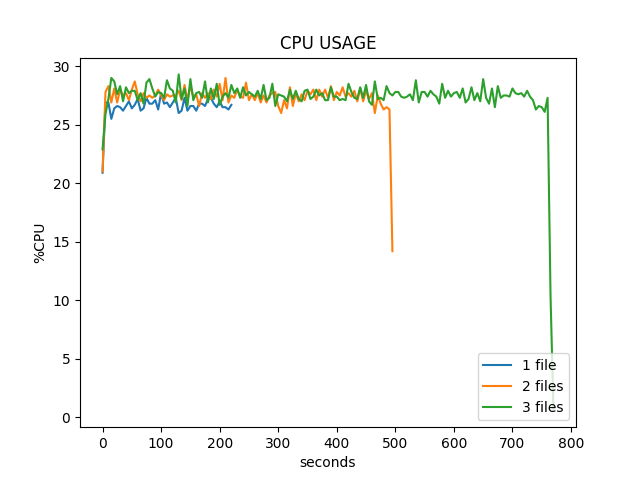
\includegraphics[width=70mm]{Figures/CPUusageImportEDFNRFILEs.png}}
        \subfigure[Buffer size]{\label{fig:EDFimportBuffer}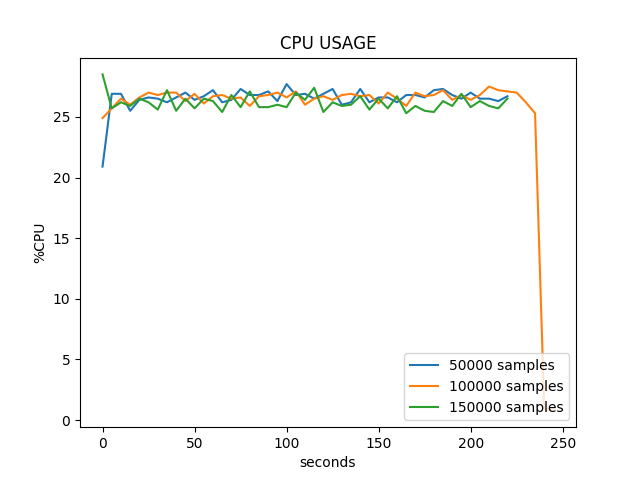
\includegraphics[width=70mm]{Figures/EDFimportBUFFlength.png}}
        \caption{CPU usage for the EDF import experiment}
        \label{fig:Figures/EDFIMPORT}
\end{figure}
When increasing the number of files that are simultaneously read, the responsive metrics are linearly increasing. Although each input file is managed by a separate thread, it must wait for accessing and writing to the database. The larger the number of file read, the longer the time to write to the database file, hence, the power consumption is increased. As presented in Figure \ref{fig:EDFimportNRfiles}, the CPU usage is increasing when the number of file reads is increased, but it is quiet stable between 25\% to 30\%. This is because the waiting time for I/O is much longer than the CPU time. In contrast, when increasing the batch size, the power consumption is decreased, because the database application reduces the overhead for writing data to the database file. However, the CPU usage is likely the same for each iteration, because the CPU time that is used to parse samples in the a01.edf file is mostly unchanged.\\
As presented in Table \ref{tab:NrOfSIMULTANEOUSELYREAD}, the EDF files are 18 times bigger when they are stored in the database file, because the EDF/EDF file formats do not include metadata in a sample while the database model includes metadata such as timestamp and the record id a sample belongs to. Moreover, each sample in a EDF file i limited to 2 bytes integer while a sample in the database is 8 bytes float. However, the metadata used in the database model provide many advantages for working with data, such as leveraging the advantages of SQL, easy to mixed multiple channels from different sources, etc.\\
The a01.edf file contains 2958000 samples, and the database application took 228235 milliseconds to insert the samples to the database. It is about 12960 samples per second. The time to read a EDF format file is therefore depending on the number of samples the file contains. The time for the reading process is decreasing when the number of samples in a EDF format file is increasing.\\
The resource usage is efficient, but the performance is poor when importing multiple EDF/EDF plus format files simultaneously. This is because the files take turn to write their data to the database file. Parallel reading files does not increase the database writing performance, but it increases the performance for parsing data from EDF files.
\section{EDF export}
The database application is required to export data to EDF file format for sharing or for backup data purposes. Since each record in the database is defined for a specific channel of a source (a.k.a channel record), and if records have the same patient id, physician id and timestamp, they are considered to be belonged to the same collecting process (a whole record). It is because a patient can use multiple sensor platforms to collect data. By choosing records with the same patient id, physician id and timestamp, a whole record can be retrieved. A user can choose which channel records to be included in the exported record, because sometimes the user needs data from some specific channels. The EDF file format requires that a whole record needs to be divided into small data records. The duration of the small data records is freely chosen. However, a data record size does not exceed 61440 bytes \citep{EDFpluss}. In the implementation of the database application, a data record is defined as a buffer in memory, and this buffer is flushed to the exported file when it is full. Hence, the data record size is also the buffer size which is defined by a summary of all channel buffer sizes. A channel buffer size is defined by multiplying the data record duration with the frequency of a channel.\\\\
$bufferSize=\sum_{i = 1}^{n}\frac{duration}{frequency\ channel(i)}$\\\\
Goals of the experiment are to evaluate the read performance of the database and resource usage such as percent CPU usage and battery consumption.
\subsection{Experiment workloads}
As presented in the design of the database application, the application continuously queries parts of a record into a buffer and writes the full buffer to the exported EDF file. The application requests database access for each selected record. If the number of selected records for exporting is large, the application needs to access the database multiple times. Therefore, the experimental workload for the experiment is the number of records to be exported.
\subsection{Experiment metrics}
A record can be very large, since it can be collected in long time, and it takes more time to export the data. The database application needs to query data multiple times to avoid memory corruption since the record cannot be kept in memory for exporting. Therefore, metrics such as CPU usage, power consumption, database read performance, and shared SQLite connect time usage are chosen as the metrics for the experiment.
\subsection{Experiment setup}
The records in the database are collected from the BITalino sensor kit during a period of 60 minutes, and all channels of the BITalino are used. Each channel delivers samples with frequency 100Hz. 
\begin{table}
\centering
\begin{tabular}{|l|c|c|c|}
\hline
\multicolumn{1}{|c|}{\cellcolor[HTML]{00D2CB}} & \multicolumn{3}{c|}{\cellcolor[HTML]{00D2CB}\begin{tabular}[c]{@{}c@{}}Experimental workload in 60 min \\ Number of exporting records\end{tabular}} \\ \cline{2-4} 
\multicolumn{1}{|c|}{\multirow{-2}{*}{\cellcolor[HTML]{00D2CB}Responsive metrics}} & \cellcolor[HTML]{00D2CB}1 (15MB) & \cellcolor[HTML]{00D2CB}3 (45MB) & \cellcolor[HTML]{00D2CB}6 (90MB) \\ \hline
\cellcolor[HTML]{00D2CB}\begin{tabular}[c]{@{}l@{}}CPU usage \\ (percent)\end{tabular} & edfFER1.txt & edfFER2.txt & edfFER3.txt \\ \hline
\cellcolor[HTML]{00D2CB}\begin{tabular}[c]{@{}l@{}}SQLite usage time \\ (millisecond)\end{tabular} & \multicolumn{1}{r|}{28 180} & \multicolumn{1}{r|}{83 271} & \multicolumn{1}{r|}{165 855} \\ \hline
\cellcolor[HTML]{00D2CB}\begin{tabular}[c]{@{}l@{}}Exported file size \\ (Megabytes)\end{tabular} & \multicolumn{1}{r|}{0.727} & \multicolumn{1}{r|}{2.13} & \multicolumn{1}{r|}{4.26} \\ \hline
\end{tabular}
\caption{Number of exporting records}
\label{tab:NrOfEXPORTINGRECORD}
\end{table}
Table \ref{tab:NrOfEXPORTINGRECORD} presents the results for the experiment where the experimental workload is the number of exporting record. The experiment is performed with 1, 3, and 6	 records for each iteration. The data record duration that is used in each iteration is five seconds. In this table, the size of collected data for each channel is equal, hence, data size in bytes for each experimental workload is calculated based on the total size of the database and number of exported channels. That is, data of six channels are stored in the database, each channel stores 15MB of data in the database.
\subsection{Results and discussion}
As presented in Table \ref{tab:NrOfEXPORTINGRECORD}, the exported files are about 22 times smaller in size compared to the size they occupy in the database. It is very efficient when the database needs to back up the data to a remote storage server, but it takes about 166 seconds to query 90MB data, or about 0,5MB per second, which is quite slow. However, the database application queries a part of the data into a buffer before writing to the exported file, the procedure is repeated multiple times until the entire record is exported. This action causes more overhead if the buffer is small. The percent CPU usage for this experiment is not so high and stable at 26\% to 27\%.
\section{Querying data experiment}
When processing a SQL query, a database management system (DBMS) goes through at least three steps. The first step is to parse the SQL query into a data structure that can be processed by the DBMS. In this step, the syntax and semantic of the query are checked to determine if the SQL statement is syntactic validity, and if the statement is meaningful, i.e., whether the columns and tables are existing in the database. The second step is to optimize the query. That is, by using a set of equivalence rules, the query optimizer can generate many equivalent plans in which a cost is assigned for each plan. The plan that has the lowest cost is taken to the third step which is to execute the query plan. Although the SQL query is optimized before querying, the complexity of the SQL query and the results from the query are not changed.\\
Goals of the experiment are to evaluate the resource usage and performance of the database application with respect to the complexity of the queries, and the size of the results.
\subsection{Experiment workloads}
In SQLite, all queries are simple select statements. A simple select statement is often processed via four steps \citep{SQLITE_SELECT}.
\begin{itemize}
\item From clause processing: The input data of the statement are specified in this step.
\item Where clause processing: The expression in the clause helps to filter the return data.
\item Group by, having processing: groups of data are calculating and aggregating with respect to the filter expression in having.
\item Distinct / ALL keyword processing: result rows are return (duplicate rows are removed if “distinct” is specified).
\end{itemize}
A compound query statement is defined via connecting multiple simple select statement by using UNION, UNION ALL, etc.\\
Workloads for the experiment are therefore depended on the FROM clause, and whether statements are compound statements. As presented in SQLite \citep{SQLITE_SELECT}, all join-operators are based on Cartesian product of the left hand side (N rows) and right hand side (M rows) of the datasets. The results from the join are therefore NxM rows. In other words, the complexity when joining two table is O(MxN). The complexity is increased by the number of tables that are stated in the FROM clause. Moreover, if the result from the query is too large to hold in the memory, the DBMS musts pass the database multiple times (multiple-passes).\\
\begin{table}
\centering
\begin{tabular}{|l|c|c|}
\hline
\cellcolor[HTML]{00D2CB}Table & \cellcolor[HTML]{00D2CB}Number of columns & \cellcolor[HTML]{00D2CB}Approximate records \\ \hline
\cellcolor[HTML]{00D2CB}SensorSource & 3 & \textless100 \\ \hline
\cellcolor[HTML]{00D2CB}Patient & 7 & \textless100 \\ \hline
\cellcolor[HTML]{00D2CB}Physician & 4 & \textless100 \\ \hline
\cellcolor[HTML]{00D2CB}Clinic & 5 & \textless100 \\ \hline
\cellcolor[HTML]{00D2CB}Person & 8 & \textless100 \\ \hline
\cellcolor[HTML]{00D2CB}Channel & 11 & \textless1000 \\ \hline
\cellcolor[HTML]{00D2CB}Record & 10 & \textless1000 \\ \hline
\cellcolor[HTML]{00D2CB}RecordAnnotation & 2 & \textless1000 \\ \hline
\cellcolor[HTML]{00D2CB}Annotation & 5 & \textless1000 \\ \hline
\cellcolor[HTML]{00D2CB}Sample & 3 & \textgreater 1 million \\ \hline
\end{tabular}
\caption{Datasets in the database}
\label{tab:dataSETs}
\end{table}
As presented in Table \ref{tab:dataSETs}, the heaviest table is the Sample table, and together with the complexity of queries, they are therefore considered the main workloads of the experiment. There are four queries that are used for evaluating the experiment; the queries are described as follow:
\begin{itemize}
\item \textbf{Query 1:} A relatively small dataset is scanned (a.k.a simple query with small result). Any tables presented in Table \ref{tab:dataSETs}, as long as not the table Sample, can be chosen for this query.
\item \textbf{Query 2:} A relatively large dataset is scanned (a.k.a simple query with large result). 
\item \textbf{Query 3:} All presented tables in Table \ref{tab:dataSETs} are joined, then an aggregate function, i.e. count, sum, max, etc., is applied to have a small result (a.k.a complex query with small result).
\item \textbf{Query 4:} All presented tables in Table \ref{tab:dataSETs} are joined, no filters are applied in this query (a.k.a complex query with large result).
\end{itemize}
\subsection{Experiment metrics}
Metrics that are used for evaluating the experiment must highlight the resource usage and performance of the database application when executing different queries with different complexity. Therefore, the metrics that are chosen for the experiment are percent CPU usage and executing time in millisecond for queries. 
\subsection{Experiment setup}
\begin{table}
\centering
\begin{tabular}{|l|l|r|r|}
\hline
\cellcolor[HTML]{00D2CB}Query nr & \multicolumn{1}{c|}{\cellcolor[HTML]{00D2CB}Table(s)} & \multicolumn{1}{c|}{\cellcolor[HTML]{00D2CB}Nr record input} & \multicolumn{1}{c|}{\cellcolor[HTML]{00D2CB}Nr record output} \\ \hline
\cellcolor[HTML]{00D2CB}1. Simple query-small result& Channel & 6 & 6 \\ \hline
\cellcolor[HTML]{00D2CB}2. Simple query-large result & Sample & 2 231 580 & 2 231 580 \\ \hline
\cellcolor[HTML]{00D2CB}3. Complex query-small result & All tables & 160 673 760 & 1 \\ \hline
\cellcolor[HTML]{00D2CB}4. Complex query-large result& All tables & 160 673 760 & 160 673 760 \\ \hline
\end{tabular}
\caption{Statistic for the queries}
\label{tab:QUERYSTATISTICS}
\end{table}
The described queries in the subsection workload of this experiment are translated into SQLite code as follow:
\begin{itemize}
\item \textbf{Query 1:} The whole table Channel is chosen to be scanned.\\\texttt{select * from Channel}
\item \textbf{Query 2:} Since the table Sample is the largest, it is chosen for this query.\\
\texttt{select * from Sample}
\item \textbf{Query 3:} This query counts number of rows return from Cartesian product all tables.\\
\texttt{select count(*) from SensorSource, Patient, Physician, Clinic, Person, Channel, Record, RecordAnnotation, Annotation, Sample}
\item \textbf{Query 4:} This query return all rows from Cartesian product all tables.\\
\texttt{select * from SensorSource, Patient, Physician, Clinic, Person, Channel, Record, RecordAnnotation, Annotation, Sample}
\end{itemize}
Table \ref{tab:QUERYSTATISTICS} presents query statistics after executing the queries, while Table \ref{tab:QUERYING} presents the results for the experiment.
\begin{table}
\centering
\begin{tabular}{|l|c|c|c|l|}
\hline
\multicolumn{1}{|c|}{\cellcolor[HTML]{00D2CB}} & \multicolumn{4}{c|}{\cellcolor[HTML]{00D2CB}Experimental workload in 60 min} \\ \cline{2-5} 
\multicolumn{1}{|c|}{\multirow{-2}{*}{\cellcolor[HTML]{00D2CB}Responsive metrics}} & \cellcolor[HTML]{00D2CB}\begin{tabular}[c]{@{}c@{}}Simple query\\ small result\end{tabular} & \cellcolor[HTML]{00D2CB}\begin{tabular}[c]{@{}c@{}}Simple query\\ large result\end{tabular} & \cellcolor[HTML]{00D2CB}\begin{tabular}[c]{@{}c@{}}Complex query\\ small result\end{tabular} & \cellcolor[HTML]{00D2CB}\begin{tabular}[c]{@{}l@{}}Complex query\\ large result\end{tabular} \\ \hline
\cellcolor[HTML]{00D2CB}\begin{tabular}[c]{@{}l@{}}CPU usage \\ (percent)\end{tabular} & Qr1.txt & Qr1.txt & Qr1.txt & \multicolumn{1}{c|}{Qr1.txt} \\ \hline
\cellcolor[HTML]{00D2CB}\begin{tabular}[c]{@{}l@{}}Executing time \\ (millisecond)\end{tabular} & \multicolumn{1}{r|}{1} & \multicolumn{1}{r|}{1 612} & \multicolumn{1}{r|}{8 958} & \multicolumn{1}{r|}{509 727} \\ \hline
\end{tabular}
\caption{Executing time and resource usage for the queries}
\label{tab:QUERYING}
\end{table}
The records in the database are collected from the BITalino sensor kit during a period of 60 minutes, and all channels of the BITalino are used. Each channel delivers samples with frequency 100Hz. 
\subsection{Results and discussion}
As presented in Table \ref{tab:QUERYSTATISTICS} and \ref{tab:QUERYING}, it takes one millisecond to scan a small dataset, which is 6 rows from the table Channel in this case. Since the dataset is very small, the main purpose of the first query in the Table \ref{tab:QUERYSTATISTICS} is to find the overhead when the database application accesses the database. To find the reading speed of the database application, a large dataset must be used, and it can be done by either scanning the entire table Sample, or Cartesian product table Sample with other tables as long as the tables have at least one row. It takes 1612 milliseconds to scan an return 2231580 rows of the table Sample; the reading speed (with all rows returned) is therefore 2231580/1612 = 1384.354 rows per millisecond or 1384354 rows per second. Likewise, the reading (with all rows returned) speed for query number four is 160673760/509727 = 315.251 or 315251 rows per second. The reading speed is decreased when increasing the number of returned rows, because when the returned data are large such that they cannot be kept in memory with one database accession, the database management system needs to access the database file multiple times. As presented in Table \ref{tab:QUERYING}, the query number three returns only one row, which means that the database management system does not need to perform many accesses to the database file. The overhead for multiple accesses is therefore removed, and the reading speed is 17936.342 rows per millisecond, or 17936342 rows per second. It is about 17936342/315251 = 56 times faster than the fourth query. Hence, with respect to the hardware platform the reading speed is mainly depending on the memory of the devices. With respect to users, algorithms that are used to get data have a huge impact on the performance of the database application. How to create a good query plan, and how to optimize SQL queries is a wide topic and therefore not to be evaluated in this section. The results from the tables show that it is quite fast to get all samples of a 60 minutes record, and the reading time is linearly increasing when the number row read is increased. Although the hardware of the mobile devices has improved, the mobile devices still can not replace stationary computers. However, these results shows that some simple queries can be performed on the mobile devices, or even some mining methods can be applied on the database before the data are sent to the stationary computer. For example, to scan and filter samples in a 60 minutes record is quiet fast (about 1.6 second) on the used mobile phone, so prefiltering data on a mobile device before sending to a stationary computer is good to be considered.\\
The percentage of CPU usage is about 3\% to 7\% for the first and the second query, but it is about three to four times higher (about 28\%) when executing the third and the fourth query. The resource usages are therefore acceptable.\\
In conclusion, if the running time for mining tasks is not critical, the database application can create threads to manage the mining tasks. The results are stored to file or sent to the physician whenever the tasks are finished. Otherwise, the raw collected data should be extracted and sent to the physician. As the results presented, time to extract data from the database is fast,i.e., about two second to get a 60 minutes record which contains six channels with 100Hz. Thus, the relation database is good to be used to store the OSA data.
\section{Stress test with visualization and mixed tasks experiment}
It is possible that a user collects data from multiple sensor sources to the database, and plots the collected data on a graph while there is an exporting process is running. In other words, the application usually performs multiple tasks simultaneously rather than finishes a task before beginning the others.\\
Therefore, the goals of this experiment are to evaluate the robustness of the database when collecting data from many different sources (both EDF files and CESAR acquisition tool), and resource usage such as CPU and battery consumption.
\subsection{Experiment setup}
Each experiment, which is presented the previous sections, is evaluated with different workloads. These workloads are increased after a certain unit of time until the application is stopped or crashed. That is, the BITalino sensor kit is connected to the database application to send its data, then multiple simulators of the CESAR acquisition tool are created and connected to the database application. While the sensor sources send their data, the a01.edf file is chosen to import into the database. Right after the file beginning to load, data that are stored from the BITalino sensor kit are chosen to export to a EDF file. After that, a random source is chosen to plot data to the graph. The tasks to connect a source, import EDF files, and export to EDF files are repeatedly performed. The experiment terminates when the application is not responding or it crashes.
\subsection{Results and discussion}
As presented in Figure \ref{fig:Figures/STRESSTEST}, the CPU usage is about 10\% with a single sensor source which has six channels and each channel sends data with 100Hz. When the second source (100Hz), the third (600 Hz) and the fourth (600 Hz) are added, the CPU usage is about 26\%, 34\%, and 45\% respectively. With importing and exporting edf files, the CPU usage reaches nearly 60\%. As presented in the figure, the CPU usage suddenly drops to 20\% after the edf files are loaded and exported. It is because the garbage collector is invoked to reclaim the usage memory. That is, when there is not enough memory space for the application, the Android operating system suspends all threads, applications with low priority (i.e., do not run in the foreground or do not have any services) are killed to get more space for the database application. With visualization, the CPU usage is about 50\% while the application collects data from the sources. The speed of incoming data and the writing speed of the database application are balanced. After that, another source is connected, the a02.edf file is imported and six random channels are selected to export. As presented in \ref{fig:Figures/STRESSTEST}, the period from the second 1500th to 2000th, the percentage of CPU usage begins to behave strange after performing these action. The reason for this behavior is the amount of data that is waiting for read/write data from/to the database, hence, these data need to be kept in memory. Because the buffer grows quite fast, the Android operating system needs to suspend all threads to claim memory. However, the Android operating system can not claim the memory usage from the buffer that is used by the database application, because the database application is running in the foreground and has services to collect data from sensor sources. Therefore, the reclaim process is repeated until the Android operating system decides to kill the application.\\
As discussed in the previous experiments, the database application can manage up to 15 BITalino sensor sources (100Hz) if only data collections are performed. For mixed tasks, the database application can manage four BITalino sensor sources, in which two sources send data with 100Hz, while the last two send data with 600Hz, which is equivalent with 14 BITalino sensor sources (100 Hz). The database application is killed by the operating system when we attempt to add one more source while importing and exporting data.\\
Data visualization has a small impact to the database application, because the CPU usage is lower than 60\% regardless plotting data to the graph or not. The performance of the database application is mainly depended on the read/write speed of the chosen database management system, SQLite in this case. Some parts of the implementation do not use background threads to get data from the database, which causes freezing the GUI if the query to get data has to wait for the other queries. For example, when users create a new record, queries to get the patient, clinic, and physician information are performed such that the users can select these information from the returned list. Moreover, in the raw query part, it must be good to prevent the users from submitting the same query if they misunderstand that the query they have submitted is not executed, because some query may take long time. Nonetheless, the implementation is a proof of concept and therefore does not take the user experiment (UX) into consideration.
\begin{figure}
    \centering
    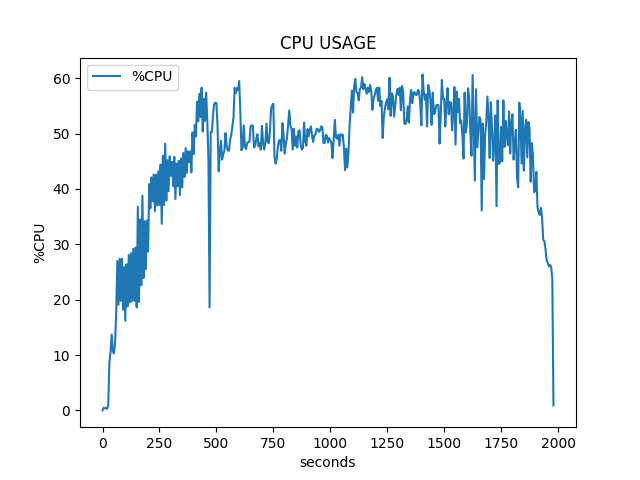
\includegraphics[width=1.0\textwidth]{Figures/StressTest.png}
    \caption{CPU usage under stress test}
    \label{fig:Figures/STRESSTEST}
\end{figure}
\section{Summary of results}
The main goals of this chapter are to convince the readers that the database design and database application meet the requirements to store OSA data, and to illustrate that a relation database solution on a mobile platform, which is used to store not only OSA data, but also other physiological data, is worth to be considered. Thus, the key results from the experiments in this chapter are presented and discussed to show that the database design and database application on a mobile platform are feasible to store OSA data, and extensible for other physiological data.\\
The database application is required to parse the incoming samples from sensor sources to tuples and store them into the database. As presented in the real time data collection experiment, the database application can continuously collect and keep data for more than 2 years for six channels with a frequency of 1Hz, or a whole day with a frequency from 100Hz to 700Hz on 20GB storage space. The percentage of power consumption is about 2.5\% which is quite efficient to use for a long time running. The overnight experiment, which uses the BITlino sensor kit where six channels with a frequency of 100Hz are used, shows that the database application consumes about 6.6\% of the total power usage, and the size of the database after collecting is 1.7GB. This means that the mobile device can store up to nine overnight records with this configuration on a 16GB SD card.\\
In case a user want to send the collected data to the physician, the collected data are exported to a EDF file which is designed to minimize the data size for sending and sharing data. The physician can import the EDF to a mobile which is implemented the database application, or can use other database analysis tools to analyze the received data from the EDF file. As presented in the import and export experiments, the data that are stored in the EDF file is about 18 times smaller as they are stored in the database, which is very efficient for sharing.\\
In some scenarios, i.e., a patient snores for a long period of time or airflow from the nose is dramatically reduced, to analyze the collected data directly on the mobile device and send the results to a stationary computer is better than just simply sending them to the stationary computer. By leveraging SQL, some mining task can be performed on the collected data, then only the results are sent to the stationary computer. As presented in the querying experiment, the query is executed fast if only few results are returned. To apply a mining task where a small set of rows is return, i.e., to find periods that are bigger than 30 seconds in which a patient snores, is good to be considered.\\
Last but not least, the stress test presents that the database application can collect data up to 84 channels (14 sensor kits, each sensor kit uses six channels to deliver data) with a frequency of 100Hz, which is possible to collect data from most of the positions on a users body and some data from environment around the user, i.e., the light, sound, etc. The collected data can also be visualized on a graph which offers users a better understand on their data.






